\section{Experimental Results}

\subsection{Generate Merkle tree}
\begin{frame}<beamer>
    \frametitle{Outline}
    \tableofcontents[currentsubsection]
\end{frame}

\begin{frame}{Experimental Results}
	\begin{table}[]
		\scriptsize
		\centering
		\begin{tabular}{crcc}
			  & Size    & File  & Directory \\
			  &			&		&		    \\
			A & 777 MB  & 48    & 6         \\
			B & 145 MB  & 54198 & 188       \\
			C & 5.95 GB & 45089 & 1459      \\
		\end{tabular}
        
		\caption{GENERATE MERKLE TREE'S TIME (IN SEC.)}
		\begin{tabular}{|c|c|c|r|}
			\hline
              & Non Hashed & Pre Hashed & Merkle tree Size \\ \hline
            A & 9.40653    & 0.00333    & 5.4 KB           \\ \hline
            B & 55.14738   & 2.70313    & 5.08 MB          \\ \hline
            C & 339.18192  & 0.3342     & 4.37 MB          \\ \hline
		\end{tabular}
        
        \caption{SERIALIZE \& DESERIALIZE MERKLE TREE OBJECT'S TIME (IN SEC.)}
		\begin{tabular}{|c|c|c|}
            \hline
              & Serialize & Deserialize \\ \hline
            A & 0.04      & 0.009       \\ \hline
            B & 0.756     & 0.299       \\ \hline
            C & 0.67      & 0.295       \\ \hline
		\end{tabular}
	\end{table}
\end{frame}

\subsection{Non POV}
\begin{frame}<beamer>
    \frametitle{Outline}
    \tableofcontents[currentsubsection]
\end{frame}

\begin{frame}{Experimental Results}{Non POV}
	\tiny
    \begin{table}[]
        \centering
        \begin{minipage}[c]{0.5\textwidth}
            \caption{The client device and SP are in the \newline same network segment}
            \begin{tabular}{lcc}
                                 & Upload (sec.) & Download (sec.) \\ \hline
                \textless 10 KB  & 0.010608      & 0.007845        \\ \hline
                \textless 100 KB & 0.014393      & 0.013691        \\ \hline
                \textless 1 MB   & 0.090440      & 0.088570        \\ \hline
                \textless 10 MB  & 0.367989      & 0.354916        \\ \hline
            \end{tabular}
            \begin{center}
                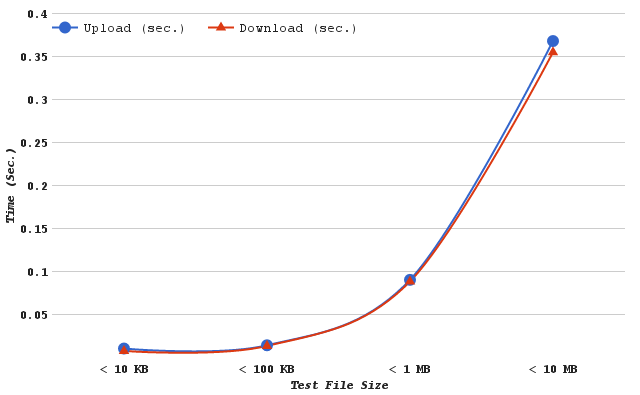
\includegraphics[width=\textwidth]{non_pov_same}
            \end{center}
        \end{minipage}%
        \begin{minipage}[c]{0.5\textwidth}
            \caption{The client device and SP are \alert{not} in the \newline same network segment}
            \begin{tabular}{lcc}
                                 & Upload (sec.) & Download (sec.) \\ \hline
                \textless 10 KB  & 0.069273      & 0.056629        \\ \hline
                \textless 100 KB & 0.121093      & 0.087351        \\ \hline
                \textless 1 MB   & 0.343584      & 0.225566        \\ \hline
                \textless 10 MB  & 1.675616      & 0.699524        \\ \hline
            \end{tabular}
            \begin{center}
                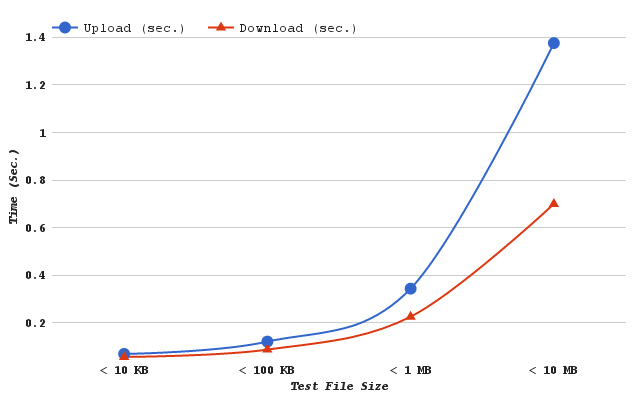
\includegraphics[width=\textwidth]{non_pov_not_same}
            \end{center}
        \end{minipage}
    \end{table}
\end{frame}

\subsection{Same Network Segment}
\begin{frame}<beamer>
    \frametitle{Outline}
    \tableofcontents[currentsubsection]
\end{frame}

\begin{frame}{Experimental Results}
{The client device and SP are in the same network segment - My Method}
	\scriptsize
    \begin{table}[]
    \centering
    \caption{THE EXECUTION TIME OF \alert{UPLOAD} OPERATIONS (IN SEC.) (Account C)}
    \begin{tabular}{lcccc}
                         & 3 Server & 5 Server & 7 Server & 9 Server \\ \hline
        \textless 10 KB  & 0.046139 & 0.067923 & 0.101676 & 0.108696 \\ \hline
        \textless 100 KB & 0.070739 & 0.083563 & 0.112895 & 0.145049 \\ \hline
        \textless 1 MB   & 0.153822 & 0.166289 & 0.200053 & 0.203870 \\ \hline
        \textless 10 MB  & 0.430937 & 0.513879 & 0.684666 & 0.694259 \\ \hline
    \end{tabular}
    \end{table}
    \begin{center}
		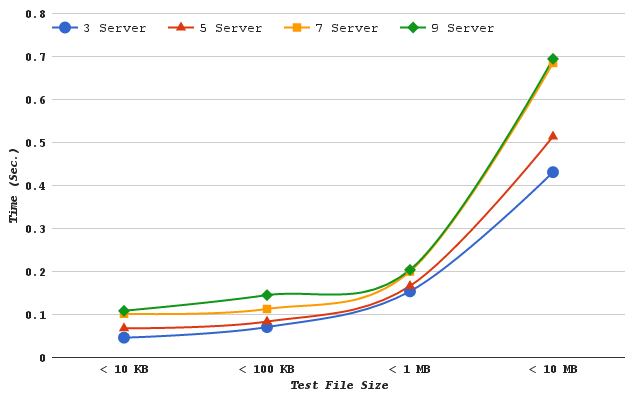
\includegraphics[width=.6\textwidth]{my_upload_same}
    \end{center}
\end{frame}

\begin{frame}{Experimental Results}
{The client device and SP are in the same network segment - My Method}
	\scriptsize
    \begin{table}[]
    \centering
    \caption{THE EXECUTION TIME OF \alert{DOWNLOAD} OPERATIONS (IN SEC.) (Account C)}
    \begin{tabular}{lcccc}
                         & 3 Server & 5 Server & 7 Server & 9 Server \\ \hline
        \textless 10 KB  & 0.042295 & 0.054263 & 0.064370 & 0.078872 \\ \hline
        \textless 100 KB & 0.053583 & 0.055442 & 0.083961 & 0.097507 \\ \hline
        \textless 1 MB   & 0.146021 & 0.159869 & 0.195817 & 0.202213 \\ \hline
        \textless 10 MB  & 0.392072 & 0.476251 & 0.622665 & 0.625499 \\ \hline
    \end{tabular}
    \end{table}
    \begin{center}
		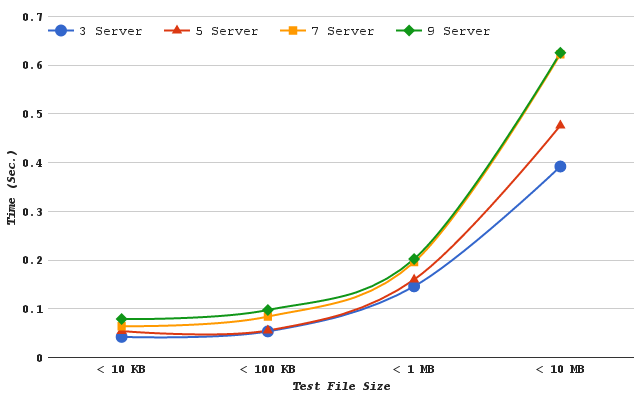
\includegraphics[width=.6\textwidth]{my_download_same}
    \end{center}
\end{frame}

\begin{frame}{Experimental Results}
{The client device and SP are in the same network segment - 2014 Cloud Com}
	\scriptsize
    \begin{table}[]
    \centering
    \caption{THE EXECUTION TIME OF \alert{UPLOAD} OPERATIONS (IN SEC.) (Account C)}
    \begin{tabular}{lccccl}
                         & sync 2   & sync 10  & sync 50  & sync 100 & sync 500 \\ \hline
        \textless 10 KB  & 0.146783 & 0.184138 & 0.332988 & 0.409002 & 0.760821  \\ \hline
        \textless 100 KB & 0.194642 & 0.209044 & 0.341408 & 0.491967 & 0.932075  \\ \hline
        \textless 1 MB   & 0.331595 & 0.385494 & 0.403481 & 0.537866 & 1.198097  \\ \hline
        \textless 10 MB  & 0.501692 & 0.518835 & 0.576403 & 0.819893 & 1.242104  \\ \hline
    \end{tabular}
    \end{table}
    \begin{center}
		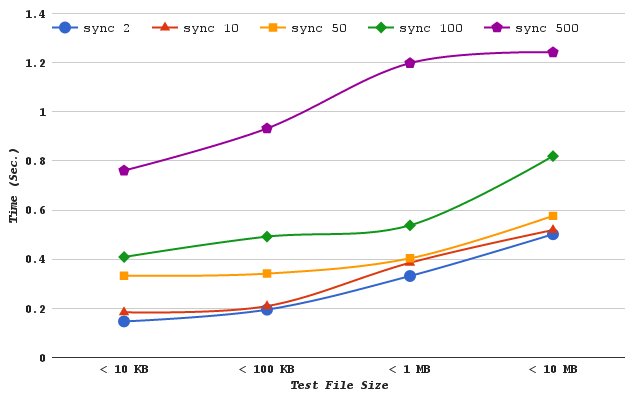
\includegraphics[width=.6\textwidth]{2014_upload_same}
    \end{center}
\end{frame}

\begin{frame}{Experimental Results}
{The client device and SP are in the same network segment - 2014 Cloud Com}
	\scriptsize
    \begin{table}[]
    \centering
    \caption{THE EXECUTION TIME OF \alert{DOWNLOAD} OPERATIONS (IN SEC.) (Account C)}
    \begin{tabular}{lccccl}
                         & sync 2   & sync 10  & sync 50  & sync 100 & sync 500  \\ \hline
        \textless 10 KB  & 0.121268 & 0.249803 & 0.331339 & 0.515956 & 1.675274  \\ \hline
        \textless 100 KB & 0.134563 & 0.258717 & 0.338794 & 0.564519 & 1.796222  \\ \hline
        \textless 1 MB   & 0.279563 & 0.302230 & 0.440841 & 0.588905 & 1.994046  \\ \hline
        \textless 10 MB  & 0.462677 & 0.539638 & 0.595140 & 1.171150 & 2.241951  \\ \hline
    \end{tabular}
    \end{table}
    \begin{center}
		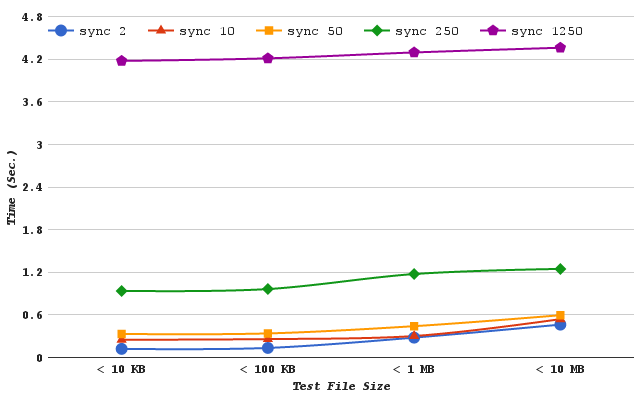
\includegraphics[width=.6\textwidth]{2014_download_same}
    \end{center}
\end{frame}

\begin{frame}{Experimental Results}
{The client device and SP are in the same network segment - UPLOAD operation}
	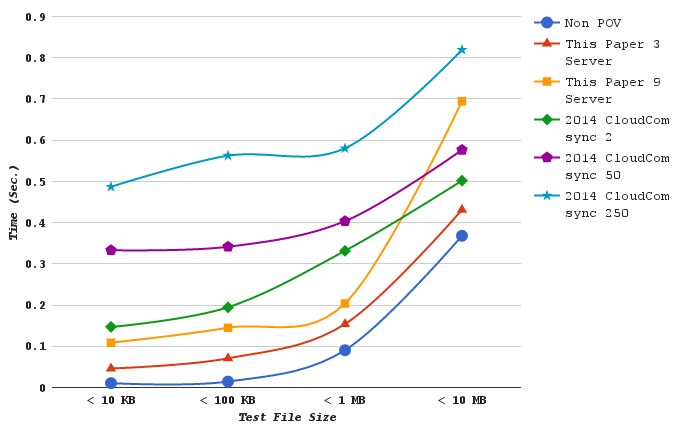
\includegraphics[width=\textwidth]{all_upload_same}
\end{frame}

\begin{frame}{Experimental Results}
{The client device and SP are in the same network segment - DOWNLOAD operation}
	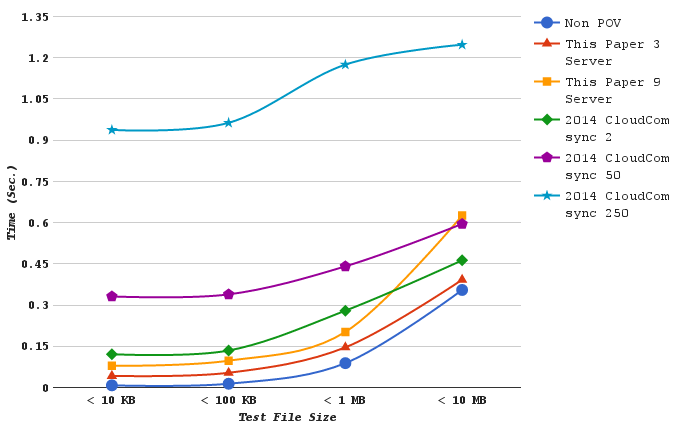
\includegraphics[width=\textwidth]{all_download_same}
\end{frame}

%TIMES
\begin{frame}{Experimental Results}
{The client device and SP are in the same network segment - UPLOAD Overhead}
	\scriptsize
    \begin{table}[]
    \centering
    \caption{My Method / Non POV (IN SEC.) (Account C)}
    \begin{tabular}{lcccc}
                         & 3 Server & 5 Server & 7 Server & 9 Server  \\ \hline
        \textless 10 KB  & 4.349552 & 6.403042 & 9.584967 & 10.246768 \\ \hline
        \textless 100 KB & 4.914887 & 5.805870 & 7.843824 & 10.077857 \\ \hline
        \textless 1 MB   & 1.700816 & 1.838656 & 2.211983 & 2.254196  \\ \hline
        \textless 10 MB  & 1.171060 & 1.396453 & 1.860562 & 1.886630  \\ \hline
    \end{tabular}
    \caption{2014 Cloud Com / Non POV (IN SEC.) (Account C)}
    \begin{tabular}{lccccl}
                         & sync 2    & sync 10   & sync 50   & sync 100 & sync 500 \\ \hline
        \textless 10 KB  & 13.837201 & 17.358624 & 31.390677 & 38.5566  & 71.7224  \\ \hline
        \textless 100 KB & 13.523544 & 14.524231 & 23.720780 & 34.1815  & 64.7598  \\ \hline
        \textless 1 MB   & 3.666447  & 4.262410  & 4.461293  & 5.9472   & 13.2474  \\ \hline
        \textless 10 MB  & 1.363336  & 1.409920  & 1.566359  & 2.2280   & 3.3754   \\ \hline
    \end{tabular}
    ~\\
    ~\\
    ~\\
    \alert{Avg: 3.97 times, Max: 6.99 times}
    \end{table}
\end{frame}

\begin{frame}{Experimental Results}
{The client device and SP are in the same network segment - DOWNLOAD Overhead}
	\scriptsize
    \begin{table}[]
    \centering
    \caption{My Method / Non POV (IN SEC.) (Account C)}
    \begin{tabular}{lcccc}
                         & 3 Server & 5 Server & 7 Server & 9 Server  \\ \hline
        \textless 10 KB  & 5.391663 & 6.917309 & 8.205786 & 10.054378 \\ \hline
        \textless 100 KB & 3.913722 & 4.049482 & 6.132484 & 7.121880  \\ \hline
        \textless 1 MB   & 1.648657 & 1.805003 & 2.210875 & 2.283095  \\ \hline
        \textless 10 MB  & 1.104689 & 1.341869 & 1.754401 & 1.762387  \\ \hline
    \end{tabular}
    \caption{2014 Cloud Com / Non POV (IN SEC.) (Account C)}
    \begin{tabular}{lccccl}
                         & sync 2    & sync 10   & sync 50   & sync 250   & sync 1250  \\ \hline
        \textless 10 KB  & 15.459033 & 31.844389 & 42.238325 & 119.489570 & 532.253193 \\ \hline
        \textless 100 KB & 9.828453  & 18.896670 & 24.745459 & 70.345135  & 307.573438 \\ \hline
        \textless 1 MB   & 3.156419  & 3.412343  & 4.977329  & 13.265056  & 48.482022  \\ \hline
        \textless 10 MB  & 1.303623  & 1.520467  & 1.676847  & 3.514280   & 12.286111  \\ \hline
    \end{tabular}
    ~\\
    ~\\
    ~\\
    \alert{Avg: 7.91 times, Max: 21.24 times}
    \end{table}
\end{frame}

\subsection{Not Same Network Segment}
\begin{frame}<beamer>
    \frametitle{Outline}
    \tableofcontents[currentsubsection]
\end{frame}

\begin{frame}{Experimental Results}
{The client device and SP are \alert{not} in the same network segment - My Method}
	\scriptsize
    \begin{table}[]
    \centering
    \caption{THE EXECUTION TIME OF \alert{UPLOAD} OPERATIONS (IN SEC.) (Account C)}
    \begin{tabular}{lcccc}
                         & 3 Server & 5 Server & 7 Server & 9 Server \\ \hline
        \textless 10 KB  & 0.217563 & 0.331341 & 0.466655 & 0.570460 \\ \hline
        \textless 100 KB & 0.245769 & 0.410174 & 0.479227 & 0.660178 \\ \hline
        \textless 1 MB   & 0.433338 & 0.594532 & 0.640597 & 0.786688 \\ \hline
        \textless 10 MB  & 1.636473 & 1.972134 & 2.011500 & 2.163858 \\ \hline
    \end{tabular}
    \end{table}
    \begin{center}
		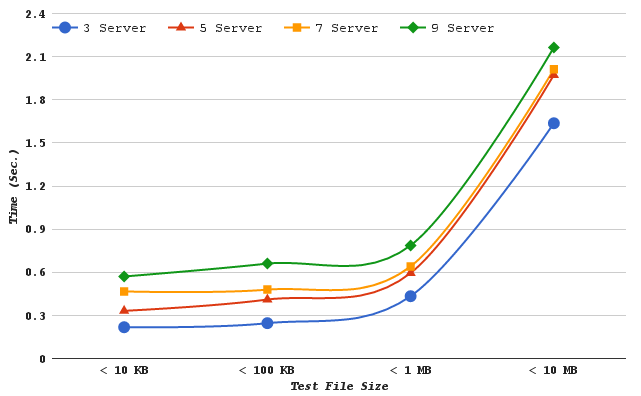
\includegraphics[width=.6\textwidth]{my_upload_not_same}
    \end{center}
\end{frame}

\begin{frame}{Experimental Results}
{The client device and SP are \alert{not} in the same network segment - My Method}
	\scriptsize
    \begin{table}[]
    \centering
    \caption{THE EXECUTION TIME OF \alert{DOWNLOAD} OPERATIONS (IN SEC.) (Account C)}
    \begin{tabular}{lcccc}
                         & 3 Server & 5 Server & 7 Server & 9 Server \\ \hline
        \textless 10 KB  & 0.263332 & 0.358435 & 0.490343 & 0.556110 \\ \hline
        \textless 100 KB & 0.270404 & 0.396497 & 0.567059 & 0.597088 \\ \hline
        \textless 1 MB   & 0.382264 & 0.590987 & 0.694622 & 0.846141 \\ \hline
        \textless 10 MB  & 0.823476 & 1.086515 & 1.208293 & 1.278169 \\ \hline
    \end{tabular}
    \end{table}
    \begin{center}
		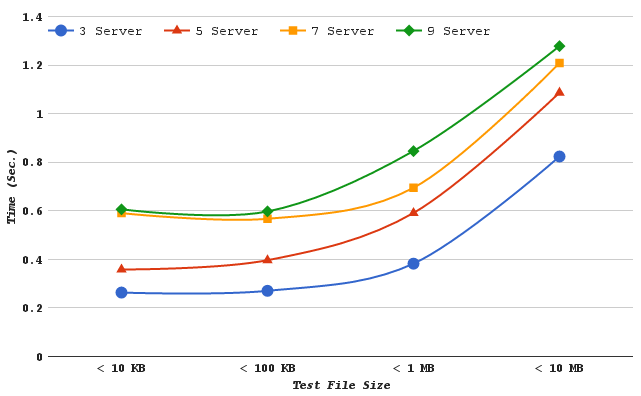
\includegraphics[width=.6\textwidth]{my_download_not_same}
    \end{center}
\end{frame}

\begin{frame}{Experimental Results}
{The client device and SP are \alert{not} in the same network segment - 2014 Cloud Com}
	\scriptsize
    \begin{table}[]
    \centering
    \caption{THE EXECUTION TIME OF \alert{UPLOAD} OPERATIONS (IN SEC.) (Account C)}
    \begin{tabular}{lccccl}
                         & sync 2   & sync 10  & sync 50  & sync 100 & sync 500  \\ \hline
        \textless 10 KB  & 0.362766 & 0.411929 & 0.486570 & 0.500776 & 1.227709  \\ \hline
        \textless 100 KB & 0.377788 & 0.416367 & 0.508769 & 0.563544 & 1.375298  \\ \hline
        \textless 1 MB   & 0.556890 & 0.619318 & 0.698361 & 0.812837 & 1.630702  \\ \hline
        \textless 10 MB  & 1.525459 & 1.882746 & 1.929606 & 1.962343 & 2.753549  \\ \hline
    \end{tabular}
    \end{table}
    \begin{center}
		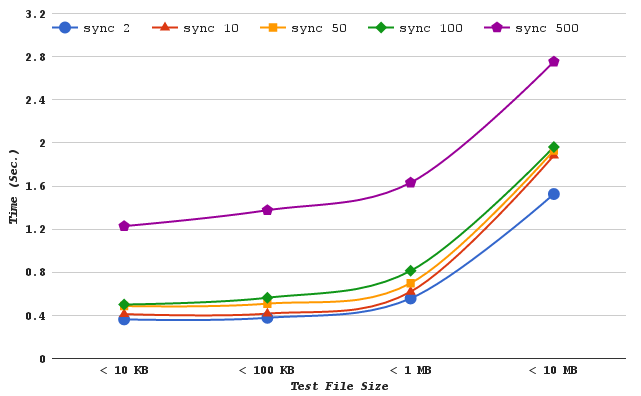
\includegraphics[width=.6\textwidth]{2014_upload_not_same}
    \end{center}
\end{frame}

\begin{frame}{Experimental Results}
{The client device and SP are \alert{not} in the same network segment - 2014 Cloud Com}
	\scriptsize
    \begin{table}[]
    \centering
    \caption{THE EXECUTION TIME OF \alert{DOWNLOAD} OPERATIONS (IN SEC.) (Account C)}
    \begin{tabular}{lccccl}
                         & sync 2   & sync 10  & sync 50  & sync 100 & sync 500  \\ \hline
        \textless 10 KB  & 0.388520 & 0.374224 & 0.524074 & 0.646150 & 2.269309  \\ \hline
        \textless 100 KB & 0.427226 & 0.440348 & 0.584122 & 0.735439 & 2.302957  \\ \hline
        \textless 1 MB   & 0.574539 & 0.687956 & 0.772134 & 0.914938 & 2.519163  \\ \hline
        \textless 10 MB  & 0.933868 & 1.024385 & 1.145598 & 1.414567 & 2.884841  \\ \hline
    \end{tabular}
    \end{table}
    \begin{center}
		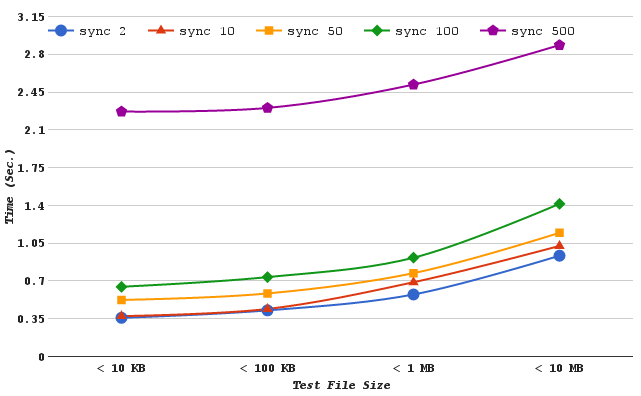
\includegraphics[width=.6\textwidth]{2014_download_not_same}
    \end{center}
\end{frame}

\begin{frame}{Experimental Results}
{The client device and SP are \alert{not} in the same network segment - UPLOAD operation}
	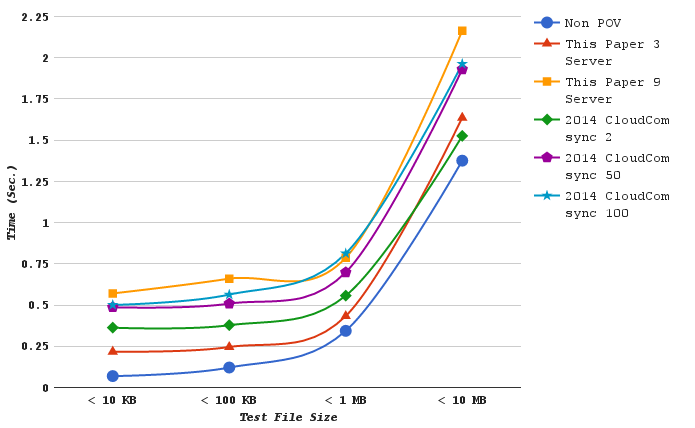
\includegraphics[width=\textwidth]{all_upload_not_same}
\end{frame}

\begin{frame}{Experimental Results}
{The client device and SP are \alert{not} in the same network segment - DOWNLOAD operation}
	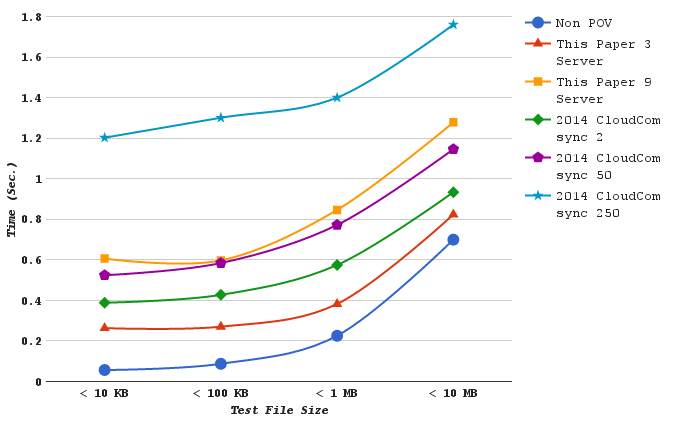
\includegraphics[width=\textwidth]{all_download_not_same}
\end{frame}

%TIMES
\begin{frame}{Experimental Results}
{The client device and SP are \alert{not} in the same network segment - UPLOAD Overhead}
	\scriptsize
    \begin{table}[]
    \centering
    \caption{My Method / Non POV (IN SEC.) (Account C)}
    \begin{tabular}{lcccc}
                         & 3 Server & 5 Server & 7 Server & 9 Server \\ \hline
        \textless 10 KB  & 3.140669 & 4.783127 & 6.736478 & 8.234973 \\ \hline
        \textless 100 KB & 2.029588 & 3.387261 & 3.957507 & 5.451819 \\ \hline
        \textless 1 MB   & 1.261228 & 1.730382 & 1.864455 & 2.289650 \\ \hline
        \textless 10 MB  & 1.189629 & 1.433637 & 1.462254 & 1.573011 \\ \hline
    \end{tabular}
    \caption{2014 Cloud Com / Non POV (IN SEC.) (Account C)}
    \begin{tabular}{lccccl}
                         & sync 2   & sync 10  & sync 50  & sync 100 & sync 500 \\ \hline
        \textless 10 KB  & 5.236767 & 5.946479 & 7.023971 & 7.2290   & 17.7228  \\ \hline
        \textless 100 KB & 3.119815 & 3.438406 & 4.201470 & 4.6538   & 11.3574  \\ \hline
        \textless 1 MB   & 1.620825 & 1.802520 & 2.032574 & 2.3658   & 4.7461   \\ \hline
        \textless 10 MB  & 1.108928 & 1.368657 & 1.402722 & 1.4265   & 2.0017   \\ \hline
    \end{tabular}
    ~\\
    ~\\
    ~\\
    \alert{Avg: 1.42 times, Max: 2.15 times}
    \end{table}
\end{frame}

\begin{frame}{Experimental Results}
{The client device and SP are \alert{not} in the same network segment - DOWNLOAD Overhead}
	\scriptsize
    \begin{table}[]
    \centering
    \caption{My Method / Non POV (IN SEC.) (Account C)}
    \begin{tabular}{lcccc}
                         & 3 Server & 5 Server & 7 Server & 9 Server \\ \hline
        \textless 10 KB  & 4.650108 & 6.329503 & 8.658827 & 9.820191 \\ \hline
        \textless 100 KB & 3.095611 & 4.539142 & 6.491742 & 6.835527 \\ \hline
        \textless 1 MB   & 1.694689 & 2.620022 & 3.079470 & 3.751199 \\ \hline
        \textless 10 MB  & 1.177195 & 1.553220 & 1.727308 & 1.827199 \\ \hline
    \end{tabular}
    \caption{2014 Cloud Com / Non POV (IN SEC.) (Account C)}
    \begin{tabular}{lccccl}
                         & sync 2   & sync 10  & sync 50  & sync 100 & sync 500 \\ \hline
        \textless 10 KB  & 6.860769 & 6.608313 & 9.254478 & 11.4102  & 40.0731  \\ \hline
        \textless 100 KB & 4.890921 & 5.041151 & 6.687090 & 8.4194   & 26.3645  \\ \hline
        \textless 1 MB   & 2.547104 & 3.049914 & 3.423100 & 4.0562   & 11.1682  \\ \hline
        \textless 10 MB  & 1.335005 & 1.464403 & 1.637682 & 2.0222   & 4.1240   \\ \hline
    \end{tabular}
    ~\\
    ~\\
    ~\\
    \alert{Avg: 1.88 times, Max: 4.08 times}
    \end{table}
\end{frame}